\documentclass[12pt]{diazessay}

\usepackage{bashful}
\usepackage{hyperref}

%----------------------------------------------------------------------------------------
%	Comment this out if you do not have `texcount` installed on your $PATH
%----------------------------------------------------------------------------------------
%\bash
%command -v texcount &> /dev/null && texcount -sum -1 csci-724-paper.tex
%\END

%Shorthand formatting commands
\newcommand{\F}[1]{$\quad$\texttt{#1}}
\newcommand{\A}{$\alpha$}
\newcommand{\B}{$\beta$}
\newcommand{\Bool   }{\texttt{Bool}}
\newcommand{\Nat    }{\texttt{Natural}}
\newcommand{\Integer}{\texttt{Integer}}
\newcommand{\Double }{\texttt{Double}}
\newcommand{\List   }{\texttt{List}}
\newcommand{\Type   }{\texttt{Type}}

%----------------------------------------------------------------------------------------
%	TITLE SECTION
%----------------------------------------------------------------------------------------

\title{\texttt{\huge{An analysis about effectiveness\\\vspace{-3mm}of structure-aware fuzzing} \\\vspace{-0.35cm} {\large A Hunter College CSCI-795 Project Proposal}\\\normalsize\url{https://github.com/recursion-ninja/Superion-YAML}}} % Title and subtitle

\author{\texttt{{\Huge Team:}\\\vspace*{-0.5em} 
		Sabina Bhuiyan \\\vspace*{-0.5em} 
		Kyoungwoo Lee \\\vspace*{-0.5em}
		Chuanyao Lin \\\vspace*{-0.25em}
		Alex Washburn}} % Author and institution

\date{\texttt{\today}} % Date, use \date{} for no date

\pagestyle{empty}

%----------------------------------------------------------------------------------------

\begin{document}

\maketitle % Print the title section

\vspace{1cm}
\section*{Abstract}

%%%%%%%%%%%%%%%%%%%%%%%%%%%%%%%%%%%%%
%   NO citations in the abstract!   %
%%%%%%%%%%%%%%%%%%%%%%%%%%%%%%%%%%%%%

In this project, we explored the efficiency of grey-box fuzzing programs with structured inputs in comparison with the ones that use generically mutated random-like inputs.
The assessment addresses testing three major file formats: JSON, Markdown, and YAML.
Of all the ubiquitous file formats, these three are currently the most popular languages that are consumed as input by a wide array of programs and have enough CVEs that we can gauge the efficacy of our fuzzing experiment.

There are some state-of-the-art fuzzers that accentuate their effectiveness with structured input such as Gramatron, Superion, and Mayhem.
We have set up the goal of evaluating the efficiency of these fuzzers on our target languages by extending their grammar support.
Excluding Mayhem, a commercial project for which we don't have access to its source code, we take two open-sourced projects; Gramatron and Superion as our extension target.
On top of that, our assessment incorporates the comparison of these two fuzzers against the other type of fuzzer.
Grimoire is a fuzzer that, without structured inputs, can perform grammar awareness fuzzing by itself.

Over the course of this project, we have attempted to extend the functionality of these two fuzzers with the intention of scrutinizing their fuzzing capabilities compared to other fuzzers like Grimoire against a corpus of CVEs of our three target file formats.
Extension and comparison of these tools proved too difficult within the time of our study.
We will discuss the difficulties presented by each tool, our attempt adapt our methodology to address these difficulties, along with the CVE replication which was achievable.

\section*{Introduction}

Fuzzing is a venerable application security testing technique developed in the late '80s\cite{Barton1988} and published in 1990\cite{Miller1990}.
Fuzzing tools generate input which is directed towards the program under test and detect if the input was accepted or caused unexpected behavior.
Such unexpected behavior can take many forms, to name a few, infinite loops, stack smashing, buffer overflows, arithmetic overflows or errors, and illegal program states.
There is a variety of Fuzzing tools\cite{ModelBasedFuzzing}\cite{GrammarBasedFuzzing}\cite{ProtocolBasedFuzzing}, each of them with input generator that mutates the input in many ways.
Different fuzzing tools tend to specialize in a few related forms of input\cite{InputDiversity} manipulation.

These fuzzing tools can be categorized into three main classes by their interaction between the fuzzer and the program under test, black-box\cite{takanen2018fuzzing}, grey-box, and white-box\cite{fuzzingsurvey}.
In a black-box scenario, the fuzzer has no knowledge of the program's internal structure and cannot use any program-specific information to direct its fuzzing efforts.
In a grey-box scenario, the fuzzer gleans information from its previous input to guide future inputs.
Lastly, in a white-box scenario, the fuzzer can utilize program analysis to inform its input generators.

There are also two broad classes of inputs generations; naive and structured\cite{fuzzingsurvey} inputs.
Naive inputs do not provide any guarantees regarding its form.
Structured inputs, on the other hand, can be defined to always preserve desired structures within their respective grammars.

AFL\cite{AFL_page}, is one of the best-known fuzzing tools. AFL relies on genetic algorithm techniques\cite{InputMutationAlgorithm} to mutate acceptable input into an input that triggers unexpected behavior.
Using the generic AFL approach, inputs would be mutated randomly, and an initially valid structured input would quickly become invalid.
But, the invalid input in this scenario, is not the one that introduces the vulnerability of the target system.
Invalid random inputs just fail to run the major part of the target system, suspended by the type checkers or the input validators.
This is a longstanding problem in the art of fuzzing and is the subject of emerging research.

Generating consistently well-structured inputs\cite{structuredInput} via "grammar-aware" mutations is one such technique for addressing the problem of randomly mutated inputs.
AFL is a poster child for efficient, naive input fuzzing.

Unexpected behavior induced by a fuzzer often reveals security flaws in the program under test.
When security flaws affect publicly available software, professional ethics dictate the responsible disclosure of said security flaw and eventually publishing a Common Vulnerabilities and Exposures (CVEs) \cite{mell2002use} report detailing the security flaw's nature and available correction(s).
The utility of CVEs is two fold.
First, they provide a method for individuals to ensure that their software is patched for all known security flaws.
Second, it facilitates security researcher's ability to replicate the detailed security flaw.
We will be making use of this second role in our project.


\section*{Motivation}
\label{Motivation}

"What is Structured Fuzzing?" In the Black Hat USA 2019\cite{blackhat2019}, the session "Going Beyond Coverage-Guided Fuzzing with Structured Fuzzing", Jonathan Metzman presented structured fuzzing and how to improve the fuzzer by adding structure awareness to it. 
Intrigued by the power of such an approach, we started our project with the goal of testing the efficiency of the well-structured inputs via "grammar-aware" mutations by improving the fuzzers we chose.

Superion\cite{superion}, 2018, is an fairly recent open source fuzzing tool created by modifying and extending AFL to produce structured inputs.
Superion currently generates valid JavaScript and XML inputs by taking a context free grammar and an input seed, then performing a series of "grammar-aware" mutations to create a sequence of validly structured inputs. The process is illustrated in the figure below.

\begin{center}
	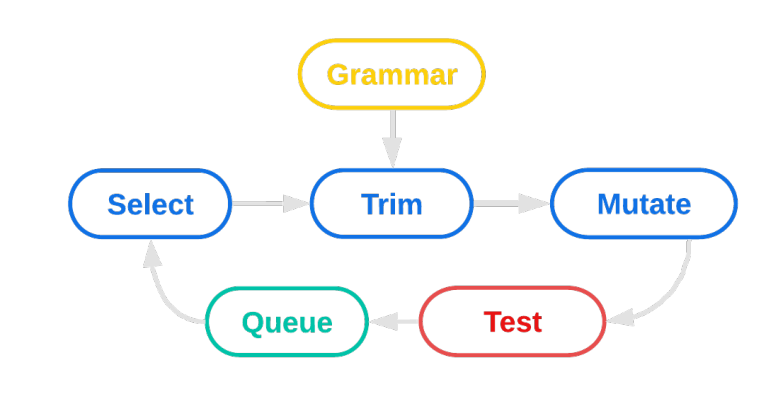
\includegraphics[scale=0.4, trim={0 1cm 0 0}, clip]{superionfig.png}\\
	\textbf{Figure 1.} Grammar-aware input generation process of Superion
\end{center}
\vspace{3mm}

Based on the context-free grammar, Superion parses each test input into an abstract syntax tree, an AST. Using ASTs, Superion introduces a grammar-aware trimming strategy that can effectively trim test inputs while keeping the input structure valid, then randomly chooses another input from AFL's queue and also parses it into AST. A sub-tree of the target input can be replaced by another sub-tree, either from the target input itself or from a randomly chosen supplementary sample. Therefore, hundreds of new samples are generated and executed to find a new path in tested programs. The results of Superion show a great increase in fuzzing efficacy when targeting programs which expect structured input.


\clearpage

Gramatron\cite{srivastava2021gramatron} is a second, and even more recent, open-source fuzzing tool designed to produce structured inputs that we decided to extend.
Released in 2021, Gramatron was designed with new mutation algorithms to increase the speed at which defects are discovered.
It does this by reducing the number of mutation steps from the input seed to trigger input mutations, rather than simply optimizing the speed at which new inputs can be generated. There are two steps in which Gramatron modifies AFL++. First, in the preprocessing phase, the context-free grammar, CFG, is converted into Greibach normal form (GNF) \cite{greibach1965new}, which is then turned into a finite state automata (FSA). This can be seen in the figure below.

\vspace{-1cm}
\begin{center}
	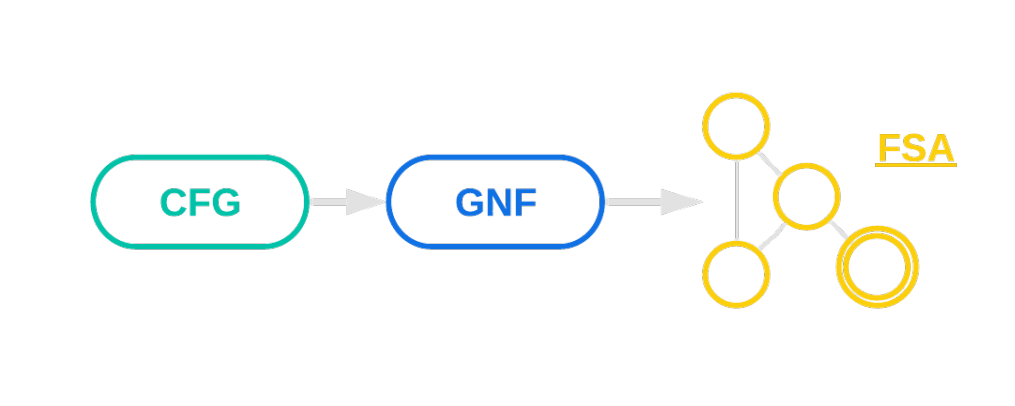
\includegraphics[scale=0.4, trim={0 3cm 0 0}, clip]{gramatronfig.png}\\
	\textbf{Figure 2.} Preprocessing phase of Gramatron
\end{center}
\vspace{6mm}

In the second step, the fuzzing phase, Gramatron uses the FSA to mutate the input into another well-formed input simply by move through transition sates of the FSA.
Given the compact and efficient nature of FSAs, each step through the transition space is constant time, and the resulting input mutation reduces to an informed string substitution.
This approach of iterative, sound mutations through a transition space is how Gramatron achieves it's exceptional speed while maintaining the desired structured fuzzing inputs.
Gramatron currently generates structured PHP and JavaScript as inputs.


Grimoire\cite{GRIMOIRE} is a structured input fuzzer which does not require an explicit structural definition to generate fuzzing inputs.
Instead, Grimoire deduces the required input structure via feedback from the target program.
Initial research suggests that this form of structure-inferring fuzz technique may be more effective than explicitly defined structured input fuzzing as Grimoire can probe corner cases much more thoroughly which are in general, excluded from formal grammars.

For a decade, AFL has been upheld as the de-facto basis of comparison for all other fuzzing techniques.
However, AFL++\cite{fioraldi2020afl++} was released as a foundational reconstruction of AFL.
AFL++ boasts integrating multiple modern fuzzing techniques, including low-frequency path prioritization previously introduced by AFLFast\cite{bohme2017coverage}, improved mutation scheduling described by MOpt\cite{lyu2019mopt}, hard byte comparison mitigation improved by LAF-Intel \cite{intel2016circumventing} and KAFL \cite{schumilo2017kafl}, as well as structured-input mutation techniques exemplified by AFLSmart \cite{pham2019smart}.
These technical improvement come with the addition of improved tool usability and robustness.
However, most notably, AFL++ has been designed with extensibility as a primary goal which is exposed via its \emph{Custom Mutator API}.
While AFL++ was not initially included in our project, it's remarkable combination extensiblity, usability, and reliability proved a truly valuable, mid-project substitution.

The goal of this project is to extend the capabilities of both Gramatron and 
Superion, then compare their performance along with Grimoire towards replicated selected CVEs.
We attempt extending the capabilities of Gramatron and Superion to support generating the three structured inputs: YAML\cite{YAMLdraft}, JSON and Markdown.
We plan to compare the efficacy of our extended versions of Gramatron and Superion to both Grimoire and previous work targeted at fuzzing these three file formats.
By utilizing the three fuzzers- Gramatron, Superion, and Grimoire- we hope to draw a rich comparison of modern fuzzing techniques.

As per the target grammar selection, aside from the fact that there is room for these formats on extending our target fuzzers, we have numerous reasons for selecting YAML, JSON, and Markdown as our extension language.
First, it has a well-defined formal grammar that allows it to be quickly and reliably integrated into the two fuzzers.
Second, these file formats are ubiquitous input formats.
This ubiquity makes our target languages a well-motivated language to extend these fuzzers to support.
Lastly, to a proper assessment of its performances, languages that have a sufficient corpus of CVEs are required. 
These languages have a decent amount CVEs that we can work with.
There are 108 (YAML), 664 (JSON), and 103 (Markdown) CVEs on MITRE\cite{MITRE}.

Although we have confined our extension targets to two cutting-edge fuzzers for various reasons, there are other modern fuzzers which could have been a suitable choice, such as; CodeAlchemist\cite{CodeAlchemist1}\cite{CodeAlchemist2}, Hawkeye\cite{Hawkeye}, Angora\cite{Angora1}\cite{Angora2}, CollAFL\cite{CollAFL}, IoTFuzzer\cite{IoTFuzzer}, RedQueen\,\cite{redqueen}, Nautilus\,\cite{Nautilus1}\cite{Nautilus2}, Periscope\cite{PeriScope1}\cite{PeriScope2}, T-Fuzz\,\cite{TFuzz1}\cite{TFuzz2}, Chopper\cite{Chopper}, QSYM\cite{QSYM1}\cite{QSYM2}, DigFuzz\cite{DigFuzz}, and FairFuzz\cite{FairFuzz1}\cite{FairFuzz2}.
All these tools are distinguished in their specialized scoped, but we have decided to work with Gramatron and Superion as these are open-sourced projects, and appear the most adaptable in generating new structured inputs.


\vspace{3mm}
\section*{Approach}

We attempted to extend the functionality of Gramatron to generate mutable, structure-aware YAML, JSON, and Markdown output.
Additionally, we attempted to extend the functionality of Superion to generate mutable, structure-aware outputs in the same three target languages.
While both projects are open source and are modular in their design for incorporating new grammars, the assessed ease of this incorporation was misguided.
Neither extension was fully successful.
However, the extension attempts did provide insightful results regarding each tool.

The usage of Grimoire as a baseline for measuring the results of Gramatron and Superion against was also unsuccessful.
There were no binaries of Grimoire available for usage and building Grimoire from source repeatedly failed due to multiple chain of dependency issues and platform specific requirements.
With the Grimoire inaccessible as a baseline metric, we substituted ALF and AFL++ to be used as our baseline metrics in anticipation of later success extending Gramatron and Superion.
When extension of Gramatron and Superion became exceedingly improbable within our time constraints, we finalized our methodology to utilize AFL as the baseline measurement and AFL++ as the structured-aware fuzzer.

We have composed a corpus of CVEs discovered from previous work.
At the time of writing, we found over 100 CVEs cataloged on MITRE\cite{MITRE} for each of target languages mentioned above.
We selected a reproducible subset of these CVEs to use as our coverage test.
Unfortunately, due to the inability to extend Gramatron and Superion, we could not use test these extensions' ability to discover the selected CVEs.
Instead we used the efficacy of AFL and AFL++ as a comparative metric.
Quantitatively, we measured the execution time of ALF and ALF++ and compare their inputs generated per second.
The motivation of this metric is to compare the computational efficiency of each tool, i.e. clock-cycles per attempt.
Qualitatively, we compare how many of the selected CVEs were rediscovered by each tool, as a determination of their general efficacy.

All the experimentations during our project are conducted on the consolidated WSL(Windows Subsystem for Linux) version 2 using ubuntu version 18.04.1.
Separate environment setup trials were done in the AWS ec2 server of the t3a.large instance.
After testing and trials on these two environments, we concluded that using WSL is a better option for us to get our expected results in a timely manner.
Although we also had another option to try the DETER server, considering the time restraints, we moved on to the next phase without testing more on research environments.
Major tasks involved in the fuzzing tests demand substantial computing power.
For that, we want to emphasize the importance of such configuration evaluations and highly recommend allocating some time to the testing environment setup if there's enough time available.

\section*{Findings}
\label{results}

\subsection*{Gramatron}

Gramatron's approach to fuzzing described above in \emph{Motivation}, while novel and efficient, is not without it's limitations.
Because the mutation mechanism is a FSA, Gramatron can only produce coverage for grammars which are regular languages.
For any grammar which is more complex than a regular language, Gramatron can only produce a structured set of strings which represent a small sub-set of the entire grammar's set of acceptable strings.
This lack of expressiveness can leave large gaps in Gramatron's coverage.
For example, some recursive, or even context-free, production rules of a grammar will need to be modified or omitted for them to be convertible to a mutation FSA.
Since Gramatron's advertised usage is on context-sensitive and Turing-complete languages, careful inspection must be taken to understand what linguistic sacrifices were made and what subset of the language Gramatron produces coverage for.

\vspace{10mm}
\hrule height 0.4mm
\begingroup \fontsize{10pt}{10pt} \selectfont \begin{alltt}
\input{JSONsource.json}
\end{alltt} \vspace{-6mm} \endgroup \hrule height 0.4mm
\vspace{6mm}
\centerline{\textbf{Figure 3.} GNF grammar specification for JSON extension}
\vspace{6mm}

The mechanism by which Gramatron takes a grammar specification and converts it into a FSA is through a pipeline of multiple grammar conversion.
First a grammar of production rules in either JSON or G4\cite{parr2013definitive} format is converted to a new set of production rules Greibach Normal Form.
This conversion is not decidable \cite{yu1997regular}.
Theoretically, if the largest production rule has $N$ non-terminals, then the GNF grammar can be represented by a push-down autamata (PDA) which, if it halts, will always halt with a stack depth of at most $N$.
However, if a GNF gramar has a recursive definition, it too is undecidable.
To be decidable, no non-terminal can transitively produce itself, i.e one must forbid productions of the (general) form $A \to B \to A$.
Once a the grammar is in GNF form, Gramatron \emph{assumes} that it is decidable and equivalent to the stack-limited, decidable PDA.
This assumption is not always sound.
Symbols are recursively substituted with their definitions.
After recursive substitution of depth $N$, all productions are in GNF form \emph{and} have at most one non-terminal per right-hand-side of a rule.
In this form, the grammar stack-limited PDA has had the potential state-space of the stack expanded out explicitly into a FSA.
This FSA is used as the mutator for Gramatron.

\vspace{10mm}
\hrule height 0.4mm
\begingroup \fontsize{10pt}{10pt} \selectfont \begin{alltt}
\input{JSONsource_automata.json}
\end{alltt} \vspace{-6mm} \endgroup \hrule height 0.4mm
\vspace{6mm}
\centerline{\textbf{Figure 4.} FSA specification for JSON extension}
\vspace{6mm}

During our extension of Gramatron to support JSON, Markdown, and YAML, we encountered numerous problems arising from the theoretical limitations above.
First, not all three of JSON, Markdown, and YAML are context free grammars with recursive definitions, and hence they cannot be directly converted to a GNF form, hence not to the FSA.
The conversion process from CFG to GNF for both grammars was fraught with infinite loops.
We dedicated substantial time to manually pre-defined both grammars in GNF to avoid the undecidability of general CFG to GNF conversion.
Subsequently, each grammar had to have it's transitive recursive form broken so that it could be converted into a FSA.
This process was also labor intensive as it require manual inspection of the grammars and elucidation as to which parts can be elided while still producing coverage for our selected CVEs.
Additionally, as part of Gramatron's internal conversion process from CFG to FSA, it disallows some characters which it considers to be special from existing within terminals and the label of non-terminals.
There is no escaping mechanism for these special characters provided by Gramatron.
One such character was the pipe (\texttt{'|'}) character, which is a required component of terminals in Markdown's definition of tables.
When special characters exist within the grammar definition, Gramatron does not provide any informative warning(s) to the user, rather it simply halts with a generic failure message.
Discovering the existence and circumvention of these special character took nearly a week of debugging Gramatron's source code.

Once Gramatron had successfully accepted our carefully tailored new grammar definitions and converted then to FSAs, we experienced a final and fatal complication.
Instead of producing structured output of either JSON, Markdown, or YAML, instead Gramatron produced binary output of an indiscernible structure.
Each of the aforementioned complications depleted our available man-hours for this project and not enough time remained to begin again th arduous process of debugging Gramatron's source code.

The results of our attempted extension of Gramatron is the assessment that Gramatron manifests a powerful and novel technique in mutation-based, structure-aware fuzzing by utilizing tenets of formal language theory to convert a CFG structure to a FSA.
However, this assessment carries with it strong disclaimers.
Currently, Gramatron is in a prototype state and not amiable for general use. 
The engineering effort required to craft a new grammar for your specific fuzzing application is almost certainly greater than the effort require to use a less structured but more refined tool, such as AFL or AFL++.
We recommend monitoring the development and applications of Gramatron over the next few years to determine if the novel mutation-based technique it exemplifies is refined and expanded into a more usable construction or incorporated into other tools.

\subsection*{Superion}

Superion is built with a specific set of supported languages at compile time.
To add a supported language to Superion, you must add a C++ lexer and parser for the desired language.
Superion will accept any lexer and parser with the appropriate interface (template), but manually writing these components in C++ is not preferable.
Instead the Superion documentation suggests defining the new grammar as a CFG in G4 format and using ANTLR\cite{parr2013definitive} to convert transpile the G4 code to C++.
The generated C++ code can then be placed on the compilation path and the new language will be added to the compilation targets of Superion when rebuilt.

Our extension of Superion to support JSON, Markdown, and YAML, encountered different technical complications.
While locating a pre-defined G4 definitions of JSON and Markdown was simple, each existing G4 definition of Markdown we found came tainted with some "flavored extension" outside of Markdown's specified definition.
Removing the extraneous portions from the Markdown G4 files we discovered proved more difficult than authoring a direct translation from the specification to the G4 format.
Once we had sufficient G4 files, we added the output from ANTLR onto Superion's compilation path.
However, we could not get the newly built Superion emit the new grammar fuzzing inputs.
We conducted a debugging effort of Superion's source code to diagnose the problem, but our effects were unsuccessful within the time limits of the semester.

\vspace{10mm}
\hrule height 0.4mm
\begingroup \fontsize{10pt}{10pt} \selectfont \begin{alltt}
\input{MarkdownParser.g4}
\end{alltt} \vspace{-6mm} \endgroup \hrule height 0.4mm
\vspace{6mm}
\centerline{\textbf{Figure 5.} Markdown parser Grammar in G4}
\vspace{6mm}

Our assessment of Superion is limited, as we were not able to successfully extend it's support for any of the attempted grammars.
The process of extension relies on the external tool ANTLR which added complexity to the extension process that could have been mitigated by a robust makefile.
Furthermore, the lack of new grammar output and feedback on correcting the behavior leaves much to be desired in terms of usability.
Ultimately Superion promises high fidelity linguistic coverage in it's structure-aware fuzzing, but we were unable to successful extend and measure these promises.

\subsection*{Grimoire}

Grimoire is build upon Redqueen, an alternative to taint checking that exploits input-to-state correspondence and overcomes fuzzing setbacks. 
Redqueen must be implemented to set up Grimoire. However, several issues arose when doing so. Redqueen had many dependency packages that did not run on our machine. 
Despite multiple attempts of installation and manually setting up our machine again so that it would be compatible with Redqueen, we failed to successfully implement the fuzzer. Debugging these errors did not suffice, and due to lack of documentation regarding these bugs, we decided to move on to AFL++ to fuzz the target programs. 
AFL++ did not have many dependencies like Grimoire did, and was much easier to implement and use. 

\subsection*{Selected target programs}


For each target language, we've selected the target programs which have already contained multiple CVEs. There are certain criteria that we decide what target programs would be useful and efficient to get started with on fuzzing.  
First, we're looking for the open source code implemented by C or C++ as the target programs.  AFL works best on C or C++ applications. When source code is available, instrumentation can be injected by a companion tool that works as a drop-in replacement for gcc or clang in any standard build process for third-party code. For example, for C++ programs, we could set CXX=/path/to/afl/afl-g++ before we compile the code. Although AFL does support instrumenting black-box binaries on the fly with QEMU, but this tends to have poor performance. 
Second, since we need a lot of time to fuzz a program, so we prefer the old version which has contained multiple CVEs. 
Third, we'll need an executable or write a simple program that reads data from stdin or from a file to fuzz the target program.  This also reflects that we need to understand the usage of the target program. Although we can fuzz the target program brute-forcedly, once we can't find any crashes, we may wonder if there are really no bugs, or we're just simply not able to pass the input seeds to the target program. 
Lastly, the target program has some functions to deal with the target language. For example, one of our target programs is YAML-CPP\cite{YAML-CPP} which is a YAML parser and emitter in C++. Finally, we choose YAML-CPP as the YAML target, MD4C\cite{MD4C} as the Markdown target, and cJSON\cite{cJSON} as the Jason target.  

The table below is a corpus of CVEs from the chosen target programs. Selected CVEs and the defective applications are shown at the bottom of each cell of \textbf{Table 1}. The numbers next to the name indicate the latest version that the defect was fixed. For example, CVE-2019-6292 can be found in the YAML-CPP version prior to 0.6.2.
\vspace{6mm}
\begin{table}[h!]
\centering
\scalebox{1} {
\begin{tabular}{V{4}l|l|lV{4}} \hlineB{3}
	\multicolumn{1}{V{4}c|}{YAML} & \multicolumn{1}{c|}{JSON} & \multicolumn{1}{cV{4}}{Markdown}  \\ \hline
	\multicolumn{1}{V{4}c|}{\begin{tabular}[c]{@{}c@{}}
		\texttt{CVE-2019-6292\cite{CVE-2019-6292}} \vspace{-2mm} \\ \footnotesize YAML-CPP < v0.6.2
	\end{tabular}} & 
	\multicolumn{1}{c|}{\begin{tabular}[c]{@{}c@{}}
		\texttt{CVE-2019-118355\cite{CVE-2019-11835}} \vspace{-2mm} \\ \footnotesize cJSON < v1.7.11
	\end{tabular}} &
	\multicolumn{1}{cV{4}}{\begin{tabular}[c]{@{}c@{}}
		\texttt{CVE-2021-30027\cite{CVE-2021-30027}} \vspace{-2mm} \\ \footnotesize MD4C < 0.4.7 
	\end{tabular}} \\ \hline
	\multicolumn{1}{V{4}c|}{\begin{tabular}[c]{@{}c@{}}
		\texttt{CVE-2019-6285\cite{CVE-2019-6285}} \vspace{-2mm} \\ \footnotesize YAML-CPP < v0.6.2
	\end{tabular}} & 
	\multicolumn{1}{c|}{\begin{tabular}[c]{@{}c@{}}
		\texttt{CVE-2019-11834\cite{CVE-2019-11834}} \vspace{-2mm} \\ \footnotesize cJSON < v1.7.11
	\end{tabular}} &
	\multicolumn{1}{cV{4}}{\begin{tabular}[c]{@{}c@{}}
		\texttt{CVE-2020-26148\cite{CVE-2020-26148}} \vspace{-2mm} \\ \footnotesize MD4C < 0.4.5
	\end{tabular}} \\ \hline
	\multicolumn{1}{V{4}c|}{\begin{tabular}[c]{@{}c@{}}
		\texttt{CVE-2018-20574\cite{CVE-2018-20574}} \vspace{-2mm} \\ \footnotesize YAML-CPP < v0.6.2
	\end{tabular}} & 
	\multicolumn{1}{c|}{\begin{tabular}[c]{@{}c@{}}
		\texttt{CVE-2019-1010239\cite{CVE-2019-1010239}} \vspace{-2mm} \\ \footnotesize cJSON < v1.7.8
	\end{tabular}} &
	\multicolumn{1}{cV{4}}{\begin{tabular}[c]{@{}c@{}}
		\texttt{CVE-2018-12112\cite{CVE-2018-12112}} \vspace{-2mm} \\ \footnotesize MD4C < 0.2.6
	\end{tabular}} \\ \hline
	\multicolumn{1}{V{4}c|}{\begin{tabular}[c]{@{}c@{}}
		\texttt{CVE-2018-20573\cite{CVE-2018-20573}} \vspace{-2mm} \\ \footnotesize YAML-CPP < v0.6.2 
	\end{tabular}} & 
	\multicolumn{1}{c|}{\begin{tabular}[c]{@{}c@{}}
		\texttt{CVE-2018-1000217\cite{CVE-2018-1000217}} \vspace{-2mm} \\ \footnotesize cJSON < v1.7.3
	\end{tabular}} &
	\multicolumn{1}{cV{4}}{\begin{tabular}[c]{@{}c@{}}
		\texttt{CVE-2018-12102\cite{CVE-2018-12102}} \vspace{-2mm} \\ \footnotesize MD4C < 0.2.6
	\end{tabular}} \\ \hline
	\multicolumn{1}{V{4}c|}{\begin{tabular}[c]{@{}c@{}}
		\texttt{CVE-2017-5950\cite{CVE-2017-5950}} \vspace{-2mm} \\ \footnotesize YAML-CPP < v0.5.3
	\end{tabular}} & 
	\multicolumn{1}{c|}{\begin{tabular}[c]{@{}c@{}}
		\texttt{CVE-2018-1000216\cite{CVE-2018-1000216}} \vspace{-2mm} \\ \footnotesize cJSON < v1.7.3
	\end{tabular}} &
	\multicolumn{1}{cV{4}}{\begin{tabular}[c]{@{}c@{}}
		\texttt{CVE-2018-11547\cite{CVE-2018-11547}} \vspace{-2mm} \\ \footnotesize MD4C < 0.2.5
	\end{tabular}} \\ \hline
	\multicolumn{1}{V{4}c|}{\begin{tabular}[c]{@{}c@{}}
		\texttt{CVE-2017-11692\cite{CVE-2017-11692}} \vspace{-2mm} \\ \footnotesize YAML-CPP < v0.5.3
	\end{tabular}} & 
	\multicolumn{1}{c|}{\begin{tabular}[c]{@{}c@{}}
		\texttt{CVE-2018-1000215\cite{CVE-2018-1000215}} \vspace{-2mm} \\ \footnotesize cJSON < v1.7.6
	\end{tabular}} &
	\multicolumn{1}{cV{4}}{\begin{tabular}[c]{@{}c@{}}
		\texttt{CVE-2018-11546\cite{CVE-2018-11546}} \vspace{-2mm} \\ \footnotesize MD4C < 0.2.5
	\end{tabular}} \\ \hline
	\multicolumn{1}{V{4}c|}{\begin{tabular}[c]{@{}c@{}}
		\texttt{} \vspace{-2mm} \\ \footnotesize 
	\end{tabular}} & 
	\multicolumn{1}{c|}{\begin{tabular}[c]{@{}c@{}}
		\texttt{CVE-2016-4303\cite{CVE-2016-4303}} \vspace{-2mm} \\ \footnotesize cJSON
	\end{tabular}} &
	\multicolumn{1}{cV{4}}{\begin{tabular}[c]{@{}c@{}}
		\texttt{CVE-2018-11545\cite{CVE-2018-11545}} \vspace{-2mm} \\ \footnotesize MD4C < 0.2.5
	\end{tabular}} \\ \hline
	\multicolumn{1}{V{4}c|}{\begin{tabular}[c]{@{}c@{}}
		\texttt{} \vspace{-2mm} \\ \footnotesize 
	\end{tabular}} & 
	\multicolumn{1}{c|}{\begin{tabular}[c]{@{}c@{}}
		\texttt{CVE-2016-10749\cite{CVE-2016-10749}} \vspace{-2mm} \\ \footnotesize cJSON
	\end{tabular}} &
	\multicolumn{1}{cV{4}}{\begin{tabular}[c]{@{}c@{}}
		\texttt{CVE-2018-11536\cite{CVE-2018-11536}} \vspace{-2mm} \\ \footnotesize MD4C < 0.2.5
	\end{tabular}} \\ \hlineB{3}
	
\end{tabular}
}
\vspace{6mm}\\ \textbf{Table 1.} Target CVEs for each languages
\end{table}

We have administered two major tasks prior to extending the functionality of each fuzzers.
First, we have set up Gramatron and Superion to run in the test environment.
The input generators for each fuzzer successfully constructed seed files \cite{superion-example}\cite{gramatron-example}that conform to the grammatic constraints of Javascript.
Configuring grammar-specific protocols and rules for extending each fuzzer was followed by the environment setup.
This was done through the course of literature review and presentation preparation, and we have built the JSON grammar definition\cite{json-source.json} for extending Gramatron.

\vspace{10mm}
\hrule height 0.4mm
\begingroup \fontsize{12pt}{12pt} \selectfont \begin{alltt}
\input{input.js}
\end{alltt} \vspace{-6mm} \endgroup \hrule height 0.4mm
\vspace{6mm}
\centerline{\textbf{Figure 6.} Input created from Grammar-aware input generators}

\subsection*{Results from AFL and AFL++}
While using AFL and AFL++ on our target programs. We implemented older versions of these two targets so that we were more likely to find crashes. We decided to run each fuzzer on each target program for 3 hours, to make the results as consistent as possible.

\vspace{10mm}
\hrule height 0.4mm
\begingroup \fontsize{12pt}{12pt} \selectfont \begin{alltt}
\input{target_setup.js}
\end{alltt} \vspace{-6mm} \endgroup \hrule height 0.4mm
\vspace{6mm}
\centerline{\textbf{Figure 7.} The example of the target program setup}
\vspace{6mm}

Mostly, the repository of the target program has provided some test cases, so we can take these as input seeds for the fuzzers.
After fuzzing the target program in a period of time, it has generated over 100 uniq crashes in both YAMLL-CPP and MD4C. 


In order to analysis these crashes files, we've tried to reproduce the known CVEs by understanding how the specific CVE is found from those discover.
For example, CVE-2017-11692\cite{CVE-2017-11692}, the description of this CVE shows string”!2” can crash the program.
So, we also found the same crash result when we pipe our crash files to the target program.
After that, we have piped different crash files into the target program, we still get same crash messages.
Since the AFL mutator will keep mutating the input file as we mentioned before, so it's reasonable that, even these crash files are unique, but the pattern might not be too much different. That's why we'll keep getting same crash message.

\vspace{3mm}
\begin{center}
	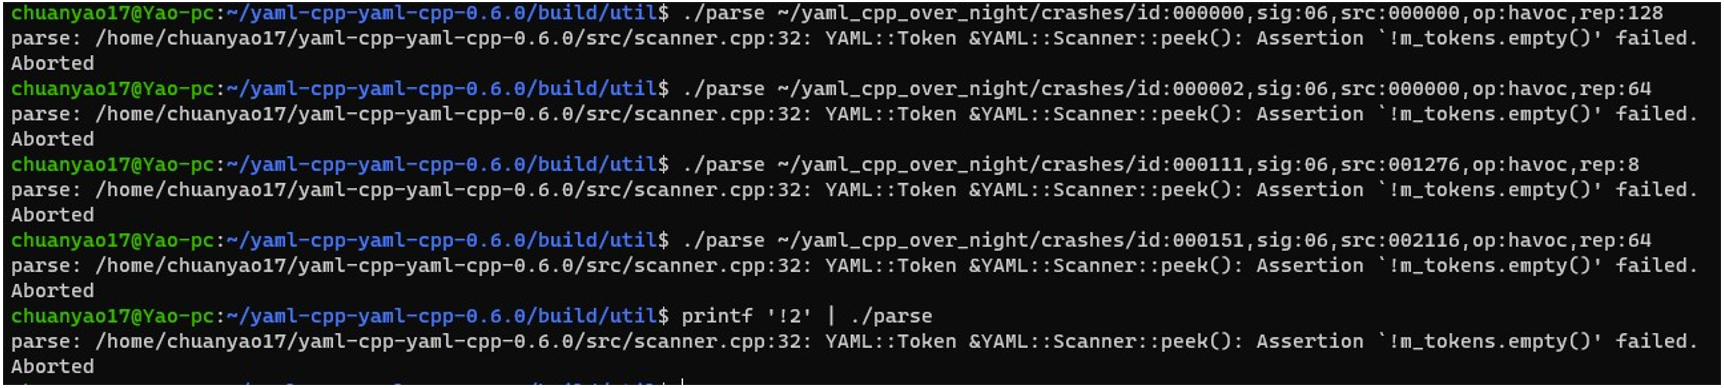
\includegraphics[scale=0.35, trim={0 0 0 0}, clip]{yaml_cpp_crashes.png}\\
	\textbf{Figure 8.} Crashes testing for YAML-CPP
\end{center}
\vspace{3mm}

For analyzing the results of MD4C, The message we can only get is the segmentation fault for testing different the crash files. So, if we want to know what's different between them, we'll need another tool to sanitize them.

\vspace{6mm}
\begin{center}
	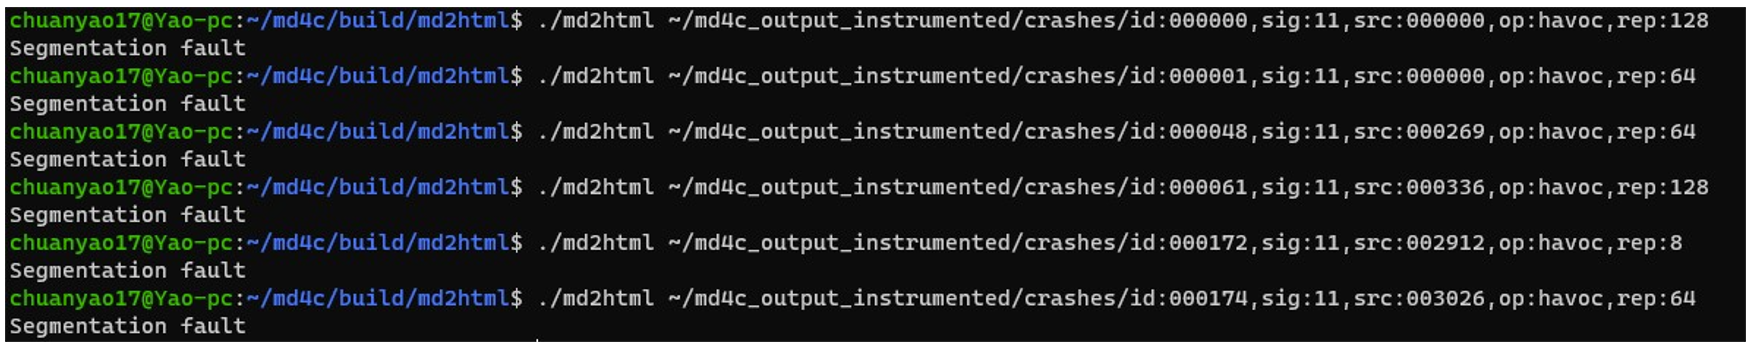
\includegraphics[scale=0.35, trim={0 0 1cm 0}, clip]{md4c_crashes.png}
	\textbf{Figure 9.} Crashes testing for MD4C
\end{center}
\vspace{3mm}

So far, these crashes are just existing flaws for the old version of the target program. We've also fuzzed the latest version of the target program, but no crashes have been found.
For the crashes files we've found, we assume that if the fuzzing time gets longer, after the fuzzer searching the target program deeply, the generated crash files might be in different pattern. Moreover, in order to specify the unique differences among them, we'll need another tool or method to know the detail reasons for how these files crash the program.

Figures in the appendix show example crashes induced by AFL++.
 
\vspace{3mm}
\begin{table}[h!]
\centering
\scalebox{1} {
\begin{tabular}{V{4}l|l|lV{4}} \hlineB{3}
	\multicolumn{1}{V{4}c|}{} & \multicolumn{1}{c|}{AFL} & \multicolumn{1}{cV{4}}{AFL++}  \\ \hline
	\multicolumn{1}{V{4}c|}{yaml-cpp} & 
	\multicolumn{1}{c|}{116} &
	\multicolumn{1}{cV{4}}{166} \\ \hline
	\multicolumn{1}{V{4}c|}{md4c} & 
	\multicolumn{1}{c|}{175} &
	\multicolumn{1}{cV{4}}{535} \\ \hlineB{3}
\end{tabular}
}
\vspace{6mm}\\ \textbf{Table 2. }Number of Crashes Found 
\end{table}
\begin{table}[h!]
\centering
\scalebox{1} {
\begin{tabular}{V{4}l|l|lV{4}} \hlineB{3}
	\multicolumn{1}{V{4}c|}{} & \multicolumn{1}{c|}{AFL} & \multicolumn{1}{cV{4}}{AFL++}  \\ \hline
	\multicolumn{1}{V{4}c|}{yaml-cpp} & 
	\multicolumn{1}{c|}{1298/sec 1cycle} &
	\multicolumn{1}{cV{4}}{2191/sec 1cycle} \\ \hline
	\multicolumn{1}{V{4}c|}{md4c} & 
	\multicolumn{1}{c|}{2855/sec 0cycle} &
	\multicolumn{1}{cV{4}}{2198/sec 2cycle} \\ \hlineB{3}
\end{tabular}
}
\vspace{6mm}\\ \textbf{Table 3. }Execution Speed 
\end{table}
\begin{table}[h!]
\centering
\scalebox{1} {
\begin{tabular}{V{4}l|l|lV{4}} \hlineB{3}
	\multicolumn{1}{V{4}c|}{} & \multicolumn{1}{c|}{AFL} & \multicolumn{1}{cV{4}}{AFL++}  \\ \hline
	\multicolumn{1}{V{4}c|}{yaml-cpp} & 
	\multicolumn{1}{c|}{1928} &
	\multicolumn{1}{cV{4}}{2382} \\ \hline
	\multicolumn{1}{V{4}c|}{md4c} & 
	\multicolumn{1}{c|}{3230} &
	\multicolumn{1}{cV{4}}{5404} \\ \hlineB{3}
\end{tabular}
}
\vspace{6mm}\\ \textbf{Table 4. }Total Paths 
\end{table}

\section*{Discussion}

Based on the fuzzing tests conducted on the selected CVEs, we found that AFL++ was much more efficient than AFL. 

When fuzzing yaml-cpp with AFL, there were a total of 116 crashes found. With AFL++, 166 crashes were found. When fuzzing markdown, AFL found a total of 175 crashes, while AFL++ found 535 crashes. For both target programs, AFL++ found more crashes than AFL. The higher number of crashes found with AFL++ indicate that the fuzzer provided more randomized inputs and found more test cases to cause a crash.

When analyzing execution speed, AFL was slower than AFL++ when fuzzing yaml-cpp, although both managed to complete one cycle, the time the fuzzer takes to pass through all the test cases in the queue. When fuzzing markdown, although AFL had a higher execution speed, AFL++ managed to complete one full cycle, while AFL did not complete any.

AFL++ completed more total paths than AFL did when fuzzing both yaml-cpp and markdown. This indicates that AFL++ explored more paths, and generated more input to reach these paths.


\section*{Future Experimentation}
For the future work, we would like to investigate the similarities between the crashes we found and the CVEs known for each target language. We think that either writing a function to parse all the crashes, or implementing another program, address sanitizers, with fuzzing would help us. Address sanitizers are used to detect bugs when fuzzing a target program. Using this modifier would aid us in investigating the crashes further.

\clearpage
\section*{Division of Labor}

Alex Washburn devised the main concept of the project.
Chuanyao Lin and Alex Washburn designed the project and derive fuzzing techniques.
Sabina Bhuiyan and Kyoungwoo Lee conducted literature reviews and related research on extending the fuzzing tools.
Kyoungwoo Lee and Alex Washburn attempted to extend Gramatron to support targeted file formats.
Alex Washburn attempted to extended Superion to support targeted languages.
Sabina Bhuiyan attempted to build and instrument Grimoire.
Chuanyao Lin Setup AFL and AFL++.
Sabina Bhuiyan, Chuanyao Lin, and Alex Washburn fuzzed targeted programs with AFL to replicate CVEs.
Sabina Bhuiyan, Chuanyao Lin, and Kyoungwoo Lee fuzzed targeted programs with AFL++ to replicate CVEs. 
Chuanyao Lin and Sabina Bhuiyan analyzed the fuzzing results of AFL and AFL++.
Kyoungwoo Lee designed and assembled the project poster.
All members authored this project report.

\section*{Timeline}

The project timeline is partially defined by the course syllabus where deadlines are concerned and partially team defined where the syllabus does not give guidance.
The following is a rough accounting of the project development:

\begin{enumerate}[label={}]
	\item \texttt{2021-08-29:} Form team and brainstorm project ideas
	\item \texttt{2021-09-05:} \textbf{Project Proposal due}
	\item \texttt{2021-09-12:} Revise and resubmit proposal
	\item \texttt{2021-09-19:} Background research \& revise \/ resubmit proposal
	\item \texttt{2021-09-26:} Background research \& revise \/ resubmit proposal
	\item \texttt{2021-10-03:} Finalize proposal, Collect and finalize CVEs corpus
	\item \texttt{2021-10-10:} \textbf{Midterm project presentations due}
	\item \texttt{2021-10-17:} \textbf{Midterm project reports due}
	\item \texttt{2021-10-24:} Initial Superion \& Gramatron extension; Grimoire setup
	\item \texttt{2021-10-31:} 
	\item \texttt{2021-11-07:} Tune 3 fuzzers instrumentation with programs under test
	\item \texttt{2021-11-14:} Replicate CVEs and document performance
	\item \texttt{2021-11-21:} Parallelize fuzzing \hfill (DETER/AWS)
	\item \texttt{2021-11-28:} Finish replication of CVEs and document
	\item \texttt{2021-12-05:} \textbf{Final project presentations due}
	\item \texttt{2021-12-12:} \textbf{Final project reports due 5:35 pm}
\end{enumerate}


\clearpage

\vspace{-6mm}
\begin{center}
	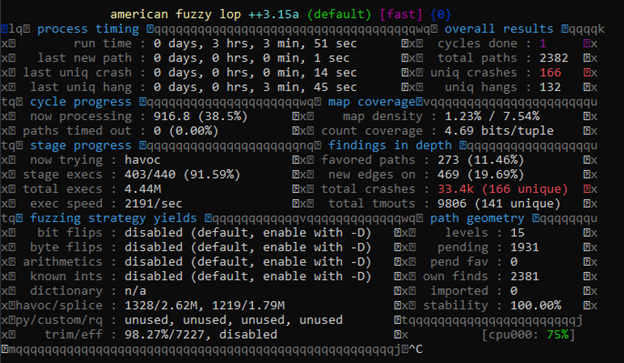
\includegraphics[scale=1.0, trim={0 0 7mm 0}, clip]{yamlfuzzer.png}\\
	\textbf{Figure 10.} Fuzzing yaml-cpp with AFL++\\
\vspace{6mm}
	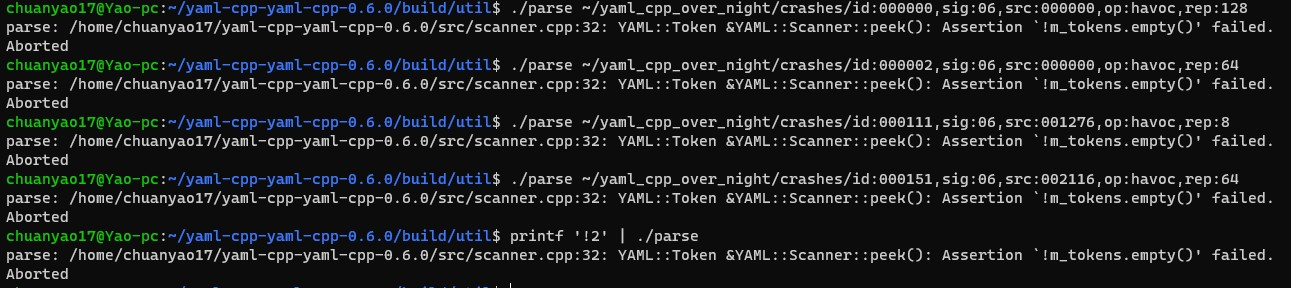
\includegraphics[scale=0.45, trim={0 3cm 0 0}, clip]{yaml_cpp_crashes.jpg}\\
	\textbf{Figure 11.} yaml-cpp crashes\\
\vspace{6mm}
	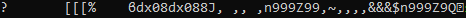
\includegraphics[scale=1.0]{yamlsamplecrashcat.png}\\
	\textbf{Figure 12.} Content of a Sample yaml-cpp crash\\
\vspace{6mm}
	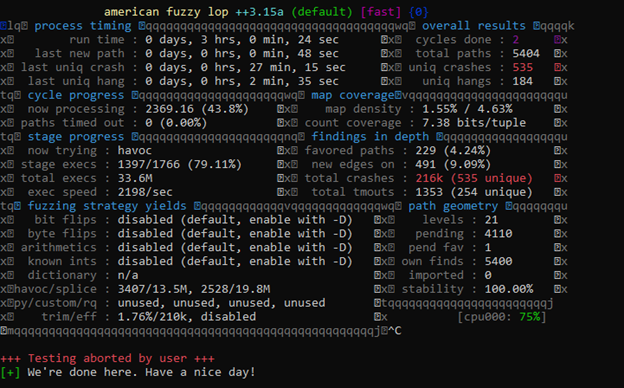
\includegraphics[scale=0.7, trim={0 0 1.5cm 0}, clip]{markdownfuzzer.png}\\
	\textbf{Figure 13.} Fuzzing markdown with AFL++ for 3 hours.\\
\end{center}
\vspace{6mm}


\begin{center}
	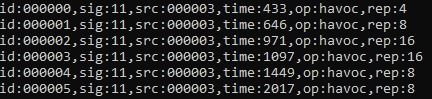
\includegraphics[scale=1.0]{markdowncrashes.png}\\
	\textbf{Figure 14.} Markdown Crashes\\
\vspace{6mm}	
	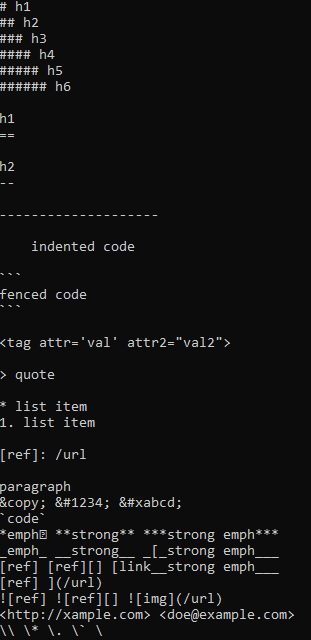
\includegraphics[scale=1.0]{markdownsamplecatcrash.png}\\
	\textbf{Figure 15.} Content of a Sample markdown crash\\
\end{center}

\clearpage

\bibliographystyle{ieeetr}
\bibliography{final-report}

\end{document}
